\documentclass[11pt]{article}
\usepackage[utf8]{inputenc}
\usepackage[T1]{fontenc}
\usepackage[margin=1in]{geometry}
\usepackage{graphicx}
\usepackage{booktabs}
\usepackage{amsmath}
\usepackage{amssymb}
\usepackage[numbers,sort&compress]{natbib}
\usepackage[hidelinks]{hyperref}
\usepackage{xcolor}
\usepackage{titlesec}
\titlespacing*{\section}{0pt}{1.1em}{0.5em}
\titlespacing*{\subsection}{0pt}{0.8em}{0.3em}

\title{\textbf{Constraint Matching: Which Brain Mechanisms Transfer\\ to a Frozen-LLM Cortex?}\\[0.4em]
\large A position paper with preliminary evidence}
\author{Lucas Savino}
\date{June 2026}

\begin{document}
\maketitle

\begin{abstract}
Brain-faithful cognitive architectures import neural mechanisms by functional analogy: the brain solves episodic memory with the hippocampus, so we port a hippocampus; it selects actions with the basal ganglia, so we port the basal ganglia. We argue this criterion is too weak, and propose a narrower one: \emph{constraint matching}. A neural mechanism can be read at two levels --- the \emph{function} it computes and the \emph{implementation} it evolved under biological constraints (spiking, low precision, noise, no global addressing, an energy budget). The rule: the presence, in the target substrate, of the constraint that motivated a mechanism is \emph{necessary --- not sufficient} --- for porting its implementation to help. On dense, high-precision compute with exact addressing --- the substrate of a frozen LLM and its adapters --- porting the function often helps; porting the implementation can be redundant or harmful when the constraint that motivated it is absent. We give five small-scale, reproducible experiments. Two validate the primitive the thesis operates on (freezing a pretrained cortex is safe when the task variable is linearly decodable, and this depends on pretraining quality). Three test the criterion: the hippocampal pattern-separation/completion micro-circuit (DG/CA3) is redundant-to-harmful on dense embeddings --- and \emph{collapses} on real LLM embeddings, where it should, by hypothesis, help least --- while a basal-ganglia reinforcement-learning mechanism (eligibility traces) helps where a frozen LLM cannot learn from reward, in a pre-registered test against a competent baseline. The contribution is a falsifiable criterion plus a cheap pre-qualification instrument (a linear probe), not a system, a novel primitive, or scale. We state our threats to validity in full; the strong, non-trivial test rests on one micro-mechanism, the evidence is toy-scale, and the rule is so far derived from cases, with a single prospective prediction.
\end{abstract}

\section{Introduction}
Using a frozen frontier LLM as an association cortex, wrapped in specialized brain-faithful modules in a predictive loop, raises an engineering question the literature rarely states precisely: \textbf{which brain mechanisms transfer to that substrate, and which do not?}

The default answer in neuro-AI is functional analogy. The brain has a circuit that solves a problem; the artificial system has the same problem; therefore port the circuit. This produced a modular inventory many groups assume similarly --- predictive cortex, episodic hippocampus, affective amygdala, RL-gated basal ganglia, cerebellar forward models, a thalamic router \citep{oreilly2016, sumers2024}. We take that inventory as a starting point, not as truth: convergence on a modular decomposition is widely assumed, but may reflect a shared metaphor as much as the brain's structure. The thesis here does not depend on the inventory being correct; it depends only on the practice of porting modules by analogy existing, which it does. What that practice lacks is a criterion for deciding, \emph{within each module}, what to port.

``The brain does X'' does not imply ``implement X the way the brain does.'' Many neural circuits are solutions to limitations of biological hardware --- noisy neurons, local communication, low precision, scarce energy --- and not the best engineering solution when you have 32-bit floats, exact inner products, and addressable memory. The idea of not confusing these levels is not new: it is Marr's levels-of-analysis argument \citep{marr1982}, and the critique of bio-plausibility as an end in itself runs through modern neuro-AI \citep{jonas2017, lillicrap2019, doerig2023}. Our contribution is not the principle. It is operationalizing it as a falsifiable test applied to a concrete substrate --- a frozen LLM plus dense adapters --- and offering, for the representational case, a cheap pre-qualification instrument.

\section{The constraint-matching criterion}
\subsection{Two levels of a neural mechanism}
Every neural mechanism can be read at two levels. The \textbf{function} is what it computes, independent of how: pattern separation orthogonalizes representations of similar items; pattern completion recovers a whole pattern from a partial cue; RL action selection learns a context-to-action map from reward. The \textbf{implementation} is \emph{how} the brain computes that function under its physical constraints. Pattern separation in the dentate gyrus (DG) is a sparse expansion with $k$-winners-take-all ($k$-WTA): it discards most dimensions because the neural substrate is noisy, low-precision, and read out by overlap-sensitive downstream cells, and sparsity buys robustness and energy efficiency \emph{there}. The levels distinction is Marr's \citep{marr1982}; what we add is a transfer criterion: an implementation is worth porting only when the constraint that motivated it is also present in the target substrate.

\subsection{Why ``constraint,'' not ``function vs.\ mechanism''}
It is tempting to summarize the thesis as ``port the function, not the mechanism.'' That fails, because the function/mechanism boundary is fluid and ``never port the mechanism'' gives the wrong verdict in an obvious case. Transformer \textbf{attention} is, formally, a neural mechanism: modern Hopfield networks are equivalent to attention \citep{ramsauer2020}, and the Hopfield network is the canonical model of CA3 pattern completion. A rule that rejected attention would be wrong --- attention is what makes the LLM cortex possible. We therefore use \textbf{constraint matching}:
\begin{quote}
The presence, in the target substrate, of the computational constraint that motivated a mechanism is \emph{necessary --- not sufficient} --- for porting its implementation to bring a performance gain. When the constraint is absent, porting the implementation does not help, and may degrade.
\end{quote}
Stated as a necessity, the rule is cleanly falsifiable: it is refuted by (a) a mechanism whose constraint is absent yet which robustly improves performance, or (b) a mechanism whose constraint is present and which fails to help even as a function. We do not claim the converse (constraint present $\Rightarrow$ implementation helps): the constraint opens the door, it does not guarantee the gain.

\paragraph{Naming ``the constraint'' without cheating.} The rule's weak point is that ``the constraint a mechanism solves'' can be named \emph{after} the verdict is known, turning prediction into rationalization. We adopt an operational definition to contain this: the constraint of a mechanism is \emph{the limitation of the biological substrate that, if removed, would make the mechanism unnecessary}. Under it, DG's constraint is ``noisy, low-precision neurons without global addressing and with limited readout''; remove it (exact floats, exact cosine) and sparsification loses its purpose. We stay honest: in the experiments below the constraint was named by us, and we have no guarantee someone else would name the same. Section~\ref{sec:threats} discusses this; the rule is, today, more explanatory than predictive, and Section~\ref{sec:e5} reports our one attempt to make it predict.

\paragraph{The status of attention/CA3.} We use attention as a \emph{sanity check}, not as evidence. Attention was not ported from the brain under the matching rule; it was already in the transformer, found by engineering, and \emph{later} shown equivalent to Hopfield. The rule is \emph{consistent} with keeping it --- it did not \emph{decide} it. The variable our experiments actually manipulate is not ``DG/CA3'' but \textbf{sparsification}: we keep CA3's completion in its dense form ($=$ attention) and discard DG's sparsity.

\section{Experiments}
All experiments are toy-scale, with multiple seeds, isolating one factor at a time, with exact numbers from the result documents in the code release. \textbf{E1--E2 validate the primitive} (freezing is viable; a linear probe predicts when). \textbf{E3--E5 test constraint matching}: E3 the absent side, E4 and E5 the present side.

\subsection{E1 --- Representation: freezing recovers co-training when the information is present}
\textbf{Setup.} A 2D reach task with a goal hidden in a ``scene,'' trained by imitation, 5 seeds. We compare end-to-end co-training; a frozen cortex plus trainable adapter under degradation modes (rich, coarse, misaligned, random, and a 1-dimensional bottleneck); and a monolith.

\textbf{Result.} With a static goal, mean success at the slow tick: co-training $1.00$, frozen-rich $1.00$, coarse $1.00$, misaligned $0.97$, random $0.99$ --- all tie co-training. Only the 1-dimensional bottleneck on a 2D goal collapses ($0.13$ success). Sweeping bottleneck capacity (Fig.~\ref{fig:e1}): success is $0.25$ at 1 dim, $1.00$ at 2/3/4 dims --- freezing fails exactly when capacity drops below the task's intrinsic dimension. A \textbf{linear probe} ($R^2$ of decoding the goal from the frozen representation) predicts this: $R^2$ $0.99$ for the conditions that succeed vs.\ $0.43$ for the bottleneck that fails.

\textbf{What it isolates.} The risk of freezing here is not ``wrong features,'' it is ``missing information.'' Any function of the input that retains at least the task's intrinsic dimension preserves the goal, and the trainable adapter reconstructs it.

\begin{figure}[t]
\centering
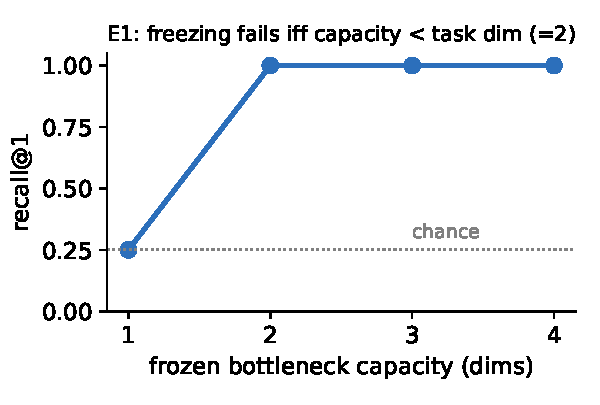
\includegraphics[width=0.45\linewidth]{figs/fig_e1.pdf}
\caption{E1: freezing a pretrained cortex costs no accuracy until the representation's capacity falls below the task's intrinsic dimension (here, 2). The boundary is sharp.}
\label{fig:e1}
\end{figure}

\subsection{E2 --- Representation quality: pretraining matters, in a real model}
\textbf{Setup.} A linear probe on a real frozen vision model (pretrained ResNet18, run on Apple Silicon). Synthetic images of a square with known position, size, and color; metric is out-of-sample $R^2$ of decoding each variable. We compare against the same deep network untrained (random weights) and a capacity curve.

\textbf{Result.} Pretrained: mean $R^2$ $0.85$ (position $0.95/0.96$). A \emph{random} deep network: mean $R^2$ $-0.44$ (worse than the mean). The capacity curve rises monotonically, $0.04 \to 0.85$ as projected dimensions grow $1 \to 4608$. A probe on frozen Qwen2.5-0.5B representations gave $R^2$ $0.87$--$0.97$, in a distinct gate-probe setup.

\textbf{What it isolates.} It corrects the shallow toy's optimism: in E1 even a \emph{random} cortex worked, because the network was shallow. In a \emph{deep} random network the variables are not linearly decodable. Pretraining quality matters --- freezing is safe if the model is genuinely pretrained, not ``any frozen network.''

\textbf{What the probe does not isolate.} In the same Qwen run, the probe passed (gate $R^2=0.89$) yet the end-to-end system \emph{failed}: an oracle collapsed to $0.38$, limited by training scale and latent dimension, not representation. \textbf{The linear probe is necessary, not sufficient.} It measures representational decodability; it does not see latency, adapter-capacity, or non-linearity failures. Reporting only the probe $R^2$ and omitting the oracle collapse would be exactly the cherry-picking this paper warns against.

\subsection{E3 --- Constraint absent $\to$ redundant/harmful: DG/CA3 do not beat RAG}
\textbf{Setup.} A causal ablation (5 seeds) of the hippocampal micro-circuit --- DG (sparse random projection $+$ $k$-WTA) and CA3 (Hopfield $=$ attention) --- against RAG (cosine over the raw embedding), in single-trial recall under cue corruption and interference. We sweep dimension, corruption, interference, and the DG sparsity $k$, and we test on \emph{both} synthetic Gaussian clusters and \emph{real} frozen LLM embeddings.

\textbf{Result (synthetic).} RAG matches or beats DG/CA3 in every regime. Under high corruption ($0.9$, $d{=}64$): RAG $0.54$, DG $0.40$, DG$+$CA3 $0.38$. In an adversarial, pro-brain-faithful regime ($d{=}16$, extreme interference, partial cue): at corruption $0.3/0.5/0.7$, RAG $0.77/0.52/0.29$ vs.\ DG $0.38/0.21/0.12$ --- $1.4$ to $2.4\times$ RAG's advantage, exactly where pattern separation should win. Sweeping $k \in \{2,5,10,25,50,100\}\%$: \emph{no} sparsity beats RAG; at $k{=}100\%$ (no $k$-WTA, DG is a random rotation) recall still falls below RAG, isolating that CA3's completion alone does not help on dense vectors.

\textbf{Result (real embeddings).} We re-ran E3 on 200 real Qwen2.5-0.5B embeddings (layer 12, 896 dims). The null is \emph{stronger}, not weaker (Fig.~\ref{fig:e3}): DG/CA3 \emph{collapses} to $0.02$--$0.04$ recall against RAG's $0.37$--$0.87$. Mechanism: the anisotropy of LLM embeddings saturates CA3's $\mathrm{softmax}(\beta X^\top \xi)$ toward a near-uniform weighting --- the metastable state that recovers the \emph{average} of the patterns, not the item. (Caveat: $\beta$ was fixed, not re-tuned for the real scale; a larger $\beta$ or whitening could reduce the collapse. The defensible claim is that out-of-the-box the brain-faithful chain fails on real embeddings where RAG is robust.)

\textbf{What it isolates.} DG's $k$-WTA discards $\sim95\%$ of dimensions --- the very information cosine uses to separate near-orthogonal vectors. On dense continuous vectors with exact cosine, the constraint that motivated DG/CA3 (noise, low precision, limited readout) is absent, and the mechanism goes from solution to dead weight.

\begin{figure}[t]
\centering
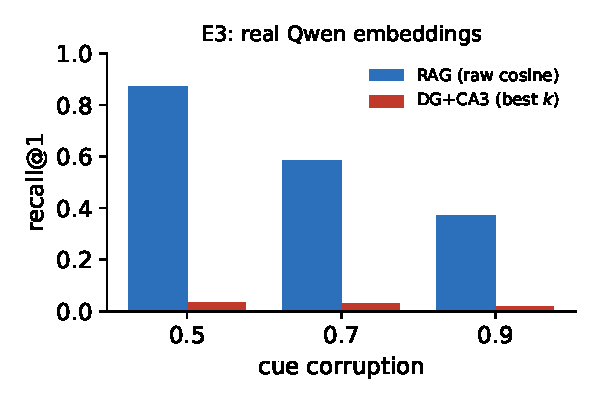
\includegraphics[width=0.45\linewidth]{figs/fig_e3.pdf}
\caption{E3 on \emph{real} frozen Qwen2.5-0.5B embeddings. The hippocampal micro-circuit (DG$+$CA3, best $k$) collapses; plain cosine retrieval (RAG) is robust. On synthetic isotropic vectors the gap is smaller; on real anisotropic embeddings the null is stronger.}
\label{fig:e3}
\end{figure}

\subsection{E4 --- Constraint present $\to$ helps (weak test): basal-ganglia RL}
\textbf{Setup.} A contextual bandit with an \emph{arbitrary} context-to-action map --- the LLM's prior cannot guess it, only online reward reveals it. 5 seeds, chance $0.25$. We compare \texttt{random}, \texttt{llm\_prior} (frozen cortex, which by construction does not receive the reward history), \texttt{bg\_rl} (tabular RL), and \texttt{oracle}.

\textbf{Result.} \texttt{llm\_prior} stays flat near chance, $0.28 \to 0.31 \to 0.30$. \texttt{bg\_rl} learns the arbitrary map, $0.27 \to 0.96$, reaching $1.00$ greedy.

\textbf{What it isolates --- and its limits.} The constraint ``learn from online reward'' is present, and the frozen LLM lacks it. But the test is \emph{weak}: it pits a learner against a non-learner on a task that only learning solves; any generic RL would win, so E4 supports the \emph{function}, not the brain-faithful implementation, against an incapable baseline.

\subsection{E5 --- Constraint present $\to$ helps (strong, pre-registered): eligibility traces}
\label{sec:e5}
\textbf{Setup.} To fix E4's weakness and the ``derived, not predictive'' charge, we pre-registered a prediction \emph{and committed it to version control before running} (the commit precedes the result commit). The brain-faithful mechanism is \textbf{eligibility traces}, TD($\lambda$) --- synaptic eligibility plus dopamine-gated plasticity. The \emph{competent} baseline is one-step TD ($\lambda{=}0$). The task is reward delayed by $K$ distractor steps; credit must cross the gap. \textbf{Pre-registered prediction:} TD($\lambda$) beats one-step TD under delay, ties without delay, and the advantage grows with $K$.

\textbf{Result (Fig.~\ref{fig:e5}).} TD($\lambda{=}0.9$) reaches $1.00$ at every gap; one-step TD drops to $0.07$--$0.30$ once $K{\geq}4$, and ties at $K{=}0$. The prediction held in direction and magnitude (TD($\lambda)\geq0.9$ vs.\ one-step $<0.6$ for all $K{\geq}4$). The sub-prediction of \emph{monotonic} growth with $K$ \textbf{failed}: the advantage is largest at $K{=}4$ and declines slightly to $K{=}24$, because one-step TD becomes \emph{less wrong} (closer to chance), not more wrong. We record this as a hit in direction and magnitude, a miss in curve shape.

\textbf{What it isolates.} A specific brain-faithful mechanism beats a \emph{competent} baseline exactly where the constraint (temporal credit assignment across a gap) is present, and ties where it is absent --- prospectively, in a single case.

\begin{figure}[t]
\centering
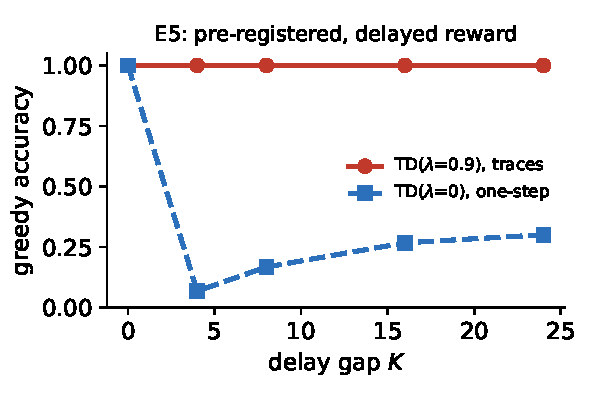
\includegraphics[width=0.45\linewidth]{figs/fig_e5.pdf}
\caption{E5, pre-registered. Eligibility traces (brain-faithful) beat a competent one-step-TD baseline under delayed reward, and tie when there is no delay ($K{=}0$, constraint absent). The prediction was committed before the run.}
\label{fig:e5}
\end{figure}

\section{The predictive rule and what each experiment supports}
The thesis reduces to a protocol. Given a candidate mechanism $X$ solving a constraint $R$: (1) name $R$ by the operational definition (the substrate limitation that, removed, makes $X$ unnecessary); (2) ask whether $R$ holds in the target substrate; (3) decide. $R$ absent $\to$ the implementation will not help (redundant at best; harmful if it actively removes something useful). $R$ present $\to$ porting the function may help; the specific implementation is a hypothesis to test. ``Absent $\to$ redundant'' and ``absent $\to$ harmful'' are different verdicts; the rule predicts only the first --- the step to ``harmful'' needs a mechanistic argument (in E3, $k$-WTA does not merely sit there, it erases dimensions cosine uses).

For representational mechanisms, the \textbf{linear probe} is a pre-qualification instrument. Linear probing as a diagnostic is not ours \citep{alain2016, hewitt2019}; we propose its use as a go/no-go gate for freezing a cortex. High $R^2$ is a verifiable \emph{necessary} condition (E1, E2); it does not guarantee end-to-end success (E2's collapsed oracle).

\begin{table}[t]
\centering\small
\begin{tabular}{@{}llll@{}}
\toprule
Point & Scope & Constraint present? & Verdict \\
\midrule
E1 & primitive + instrument & yes, if variable decodable & freezing costs no accuracy \\
E2 & primitive + instrument & yes (pretrained); no (random) & pretraining matters; probe necessary \\
E3 & matching, absent side & \textbf{no} (dense, exact cosine) & port = redundant/harmful (collapses on real) \\
E4 & matching, present (weak) & \textbf{yes} (no online learning) & RL function helps; baseline incapable \\
E5 & matching, present (strong) & \textbf{yes} (delayed credit) & traces beat competent baseline; pre-registered \\
\bottomrule
\end{tabular}
\caption{The five points and what each supports. The evidence is not a clean $2{\times}2$: E1/E2 validate the primitive, E3 tests the absent side against a strong baseline, E4/E5 the present side. The strong absent-side test rests on one micro-mechanism (DG/CA3).}
\end{table}

\section{Threats to validity}
\label{sec:threats}
The thesis's force depends on these being visible.
\textbf{Toy scale.} Five experiments, small and partly synthetic. \textbf{$n{=}1$ on the strong test.} The falsifiable, non-trivial claim (``constraint absent $\to$ do not port'') was tested causally on one micro-mechanism, DG/CA3. \textbf{Real-embedding caveat.} E3's collapse on real Qwen embeddings is partly an untuned $\beta$/anisotropy interaction; with whitening or tuned $\beta$ it could improve, though it would still have to beat exact cosine. \textbf{One pre-registration.} E5 is a single prospective prediction, not a program, and it tests the function (TD($\lambda$) \emph{is} the mechanism), not a striatal implementation; its curve-shape sub-prediction missed. \textbf{Descriptive statistics.} E3/E4/E5 report means; ``robust over 5 seeds'' means robustness to seed noise, not a significance test. \textbf{Accuracy, not energy.} E3 concludes sparsity destroys signal \emph{for recall accuracy on dense vectors}; sparsity has real value on neuromorphic hardware, which we did not measure. \textbf{The constraint can be changed on purpose.} E3 uses exact append-only memory, which \emph{removes} the constraint DG would solve; under bounded memory or online associative learning, pattern separation can matter again --- consistent with the thesis, provided the constraint is named before the result. \textbf{Falsifiability of ``the constraint.''} For any known verdict one can name a constraint that explains it; the operational definition contains part of this risk, not all. The rule was derived from cases; only E5 was prospective. \textbf{Confirmation bias.} We designed every experiment, and three confirm the architectural bet; E5 mitigates by testing the side the thesis could fail on, but independent replication is needed.

\section{Related work}
\textbf{The principle's lineage.} That neural mechanisms solve substrate constraints and should not be ported when the constraint disappears is in Marr \citep{marr1982} and in the bio-plausibility critique of modern neuro-AI \citep{jonas2017, lillicrap2019, doerig2023}. Our delta is operationalizing it as a two-sided test on a concrete substrate, plus the probe-as-freezing-gate.
\textbf{Frozen-LM conditioning.} ``Frozen LLM $+$ trainable modules'' has names and benchmarks (Voyager, Generative Agents, Reflexion). Our contribution is not the primitive --- it is the criterion for \emph{what to port inside} those modules.
\textbf{EM-LLM / HippoRAG.} EM-LLM \citep{fountas2025} segments context by Bayesian surprise and retrieves by similarity and temporal contiguity, beating RAG (authors' numbers, no independent replication). HippoRAG \citep{gutierrez2024} runs Personalized PageRank over a knowledge graph inspired by the hippocampal index. Both are \emph{allies}: they port the \emph{organization} (index, contiguity) and work; neither ports the sparse DG/CA3 micro-circuit. Our E3 tests what they assume without isolating. The raw finding (dense retrieval beats structured sparse memory) has precedent in the sparse-distributed-memory/attention comparison \citep{bricken2021}; our contribution is the neuro-specific causal framing.
\textbf{Global Latent Workspace.} \citet{devillers2024} freeze encoders and learn the bridge by contrastive plus cycle-consistency losses; they converge with us on ``freeze the expensive component, learn the routing,'' focusing the inter-space bridge where we focus which internal mechanisms to port.
\textbf{Honest positioning.} We do not claim novelty in the primitive, in system-level episodic memory, in the modular inventory, or in the levels principle. We claim something smaller and defensible: a falsifiable criterion --- constraint matching --- operationalized for a concrete substrate, plus the linear probe as a freezing gate.

\section{Conclusion}
Importing brain mechanisms by functional analogy conflates two levels: the function a circuit computes and the implementation it evolved under biological constraints. We propose a transfer criterion --- the constraint that motivated a mechanism must be present in the substrate for porting its implementation to help, a necessary not sufficient condition. Five toy-scale experiments support distinct parts: freezing a pretrained cortex costs no accuracy when the representation retains the task variable, and a linear probe predicts it cheaply but is not sufficient (E1, E2); the DG/CA3 micro-circuit is redundant-to-harmful on dense vectors, collapsing on real LLM embeddings (E3); and basal-ganglia RL helps where a frozen LLM cannot learn from reward, in a pre-registered test against a competent baseline (E5). We calibrate to what the data support: the strong test has $n{=}1$ mechanism, on synthetic and real vectors; E5 is one prospective prediction whose curve-shape sub-claim missed; the rule was derived from cases. What remains, after discounting all of this, is a criterion that makes the decision to port a mechanism \emph{falsifiable} rather than rhetorical, and that localizes the ambiguity at a concrete point: what is the constraint, is it present, is it probe-measurable. The next step is to make the rule predict and not only explain --- pre-register predictions for untested mechanisms, and take the probe to a real-scale substrate.

\section*{Acknowledgments}
This work was developed in collaboration with an AI research assistant (Anthropic's Claude), which contributed to experiment design, implementation, analysis, and drafting under the author's direction. All claims, code, and results are the author's responsibility.

\section*{Code and data availability}
All code, experiments, and result logs are available at \url{https://github.com/savinoo/brain-constraint-matching}.

\bibliographystyle{plainnat}
\bibliography{refs}

\end{document}
